\section{Background}
%TODO add some diagrams to explain more on this
%TODO every paragraph should have heading like DangNull.

% Dangling pointer information.
Dangling pointer is created when the memory object is freed. Dangling pointer is exploitable only when it is accessed. Moreover, attacker needs control over the freed memory where dangling pointer points. Attacker can place desired data in the controlled freed memory. Based on the context in which dangling pointer is used, a particular exploit can be triggered~\cite{CVEMitre, NVDNist}. The time between dangling pointer creation and use is highly important for the exploit. Longer the time period, more the chances to exploit~\cite{danglingptrfun, caballero2012undangle}.  Double free is a variation of use-after-free. Double free may corrupt memory allocator chunk information making system vulnerable. Dangling pointers are highly severe than spatial memory errors like, buffer overflow. Much of the research has happened to develop sophisticated buffer overflow mitigation techniques. Thus, spatial memory error vulnerabilities are hard to exploit. Due to this, dangling pointer vulnerabilities have gained popularity among attackers. However, mitigation techniques for dangling pointers are incomplete or incur high performance overhead. \\

% Mitigation technique : Static and dynamic analysis and its drawback.
Mitigation techniques include static analysis or run-time analysis. Static analysis   on the source code or binary is hard~\cite{feist2014statically}. It needs precise points-to analysis, type information, inter-procedural analysis. Moreover, object allocation, pointer propagation and object deallocation can occur at different places (functions, modules, threads) in the code. This further adds complexity to find accurate dangling pointers. On the other hand, dynamic analysis build pointer-object relationship during run-time. Pointer-object relationship is stored in object metadata (shadow object). Although, dynamic analysis is more accurate (low false positive and false negative rate) than static analysis, it incurs high performance overhead. Mostly, metadata lookups (i.e. finding metadata given an object or a pointer) are costly. \\

% Dynamic analysis: Why metadata management is required.
Dynamic analysis technique requires extra memory. This memory stores metadata associated with objects. Most of the schemes require object or pointer to metadata lookup. Metadata lookup should efficiently support object range lookups (i.e. finding metadata given any inbound object address). \dangnull{} uses variant of red-black tree to store metadata. Tree node is a shadow object associated with an object. Every node stores root address and size information. This bound information is needed for fast range lookups. However, metadata lookup time is highly variable. That is, it depends on the height of the shadow tree. On the other hand, \freesentry{} uses label based system~\cite{younan2010paricheck}. Label based system store unique labels in the shadow memory for each fixed size object field. Object may have multiple fixed size entries in the label table. Each entry will have same label. During metadata lookup, unique label is searched in the label table. This unique label is used as index in the object lookup hash table. However, \freesentry{} need to store more than one objects per entry in the object lookup table. Therefore, it may also have variable lookup time for the object metadata. \\

% Second data structure explanation.
Furthermore, pointer to object metadata lookup is required during pointer propagation (i.e. tracking pointer information in object metadata). \dangnull{} stores incoming and outgoing links in the shadow node along with bound information. Incoming link denotes that the object is pointed by other object and outgoing link denotes that the object is pointing to other object. \dangnull{} retrieves shadow object representing pointer address. It checks and modifies outgoing link of this object to point to other shadow object (i.e. to the object pointed by the pointer). Similarly, it modifies incoming link of the other shadow object. It has variable metadata retrieval time. \freesentry{} uses pointer lookup hash table to retrieve pointer information. Pointer lookup table does not require range lookups. Thus, hashtable is a valid choice. \freesentry{} requires huge memory for label table (almost equal to process memory), object and pointer lookup tables. Moreover, shadow memory data structure has to be thread-safe. Large number of pointer propagations, object allocations and deallocations in multi-threaded application will drastically slow down application performance. Thus, synchronizing operations on data structures increase performance overhead. \dangnull{} protects data structure using mutexes. However, \freesentry{} has not focussed on thread-safety. In \freesentry{}, object and pointer lookup hash tables need to be protected. This can be achieved having a coarse-grain or a fine-grain per-hash table entry lock.  \\

% 1) Explain metalloc. How it is suitable?. 
Any dangling pointer detection scheme (dynamic analysis) requires efficient metadata management (i.e. fast metadata allocation and retrieval strategy), thread-safety and low memory overhead. \metalloc{}~\cite{istvan2016metalloc} is an efficient and practical memory shadowing framework. It is based on the strategy that every object in the same memory page has same alignment. Thus, it maintains metadata information per page instead of per memory object. Given a pointer, it first finds corresponding page information i.e. metadata base address and alignment information. Next, it  calculates pointer offset within the page. The offset and alignment information is used to find corresponding entry in the metadata area. Therefore, it has fixed metadata lookup time for any object address range. Moreover, it provides uniform metadata tracking for all the objects (Heap, Stack and Global). Most importantly, it incurs only $1.2\%$ average run-time performance overhead for SPEC2006 benchmarks. Low performance overhead and memory optimized design along with easy to use framework makes \metalloc{} an ideal choice for implementing dangling pointer prevention scheme. \\

% 2) How freesentry desing can be achieved.
We implemented \freesentry{} scheme using \metalloc{}. \metalloc{} provides efficient object-to-metadata mapping. Therefore, we do not need Label table to fetch metadata associated with the objects. Object metadata stores a pointer to the pointer list (i.e. list of pointers information that are pointing to the object). Thus, we do not need object lookup table. Fetching a pointer information corresponding to an object requires fixed retrieval time. Next, we use pointer lookup hash table similar to \freesentry{}. Pointer-to-object metadata is retrieved using pointer lookup table. Each entry in the pointer lookup table is a doubly list of pointer information. This pointer information is also a node in the object metadata list. Thus, given a pointer, fetching an object pointer list is just finding the correct pointer information in the pointer lookup table. We evaluated this design for SPEC2006 benchmarks. We performed experiments on $64$-bit CentOS Linux with Intel Xeon CPU E5-$2640$ v$3$. We implemented LLVM compiler pass to insert run-time pointer tracking function. \\ 

\begin{figure}[t]
\center
  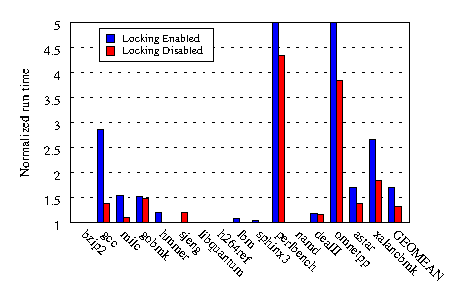
\includegraphics[width=3in]{plots/metalloc_freesentry.eps}
  \caption{SPEC2006 performance overhead for \freesentry{} scheme using \metalloc{}. Locking enabled and disabled represents normalized numbers with and without thread-safety, respectively.}
  \label{fig:metalloc-freesentry-graph}
  \vspace{-1em}
\end{figure} 

Figure~\ref{fig:metalloc-freesentry-graph}\ shows SPEC2006 run-time overhead for \freesentry{} design using \metalloc{}. It depicts normalized (with baseline) numbers with and without thread-safety. With thread-safety, run-time overhead on an average (geometric mean) is $69.6\%$. We used pthread mutexes to protect object pointer list and pointer lookup table. Without thread-safety, run-time overhead is just $33.2\%$. This number matches with the average \freesentry{} performance overhead when implemented on LLVM~\cite{freesentrypppt}. However, all our bechmarks are SPEC2006 whereas \freesentry{} has mix of SPEC2000 and SPEC2006. Moreover, our average number includes \texttt{omnetpp} run-time which has huge overhead. That is, \texttt{omnetpp} number further increases average value compared to \freesentry{}. In conclusion, \metalloc{} seem to perform better than Label based system used in \freesentry{}. Also, it has low memory overhead. However, introducing thread-safety dramatically increases performance overhead, making it impractical in production environment.
% 3) Explain graph.
% 4) Explain need for other design. 


